\documentclass[prb,preprint]{revtex4-1} 
% The line above defines the type of LaTeX document.
% Note that AJP uses the same style as Phys. Rev. B (prb).

\usepackage{amsmath}  % needed for \tfrac, \bmatrix, etc.
\usepackage{amsfonts} % needed for bold Greek, Fraktur, and blackboard bold
\usepackage{graphicx} % needed for figures
\usepackage{tabularx}

\begin{document}

\title{Double-Slit Experiment \LaTeX}
% In a long title you can use \\ to force a line break at a certain location.

\author{Yumeng Melody Cao}
\email{mcao@smith.edu} % optional
% If there were a second author at the same address, we would put another 
% \author{} statement here.  Don't combine multiple authors in a single
% \author statement.
\affiliation{Department of Physics, Smith College, Northampton, MA 01063}
% Please provide a full mailing address here.

\author{He Claudia Yun}
\email{hyun@smith.edu}
\affiliation{Department of Physics, Smith College, Northampton, MA 01063}

% See the REVTeX documentation for more examples of author and affiliation lists.

\date{\today}

%____________abstract____________________________________________

\begin{abstract}
In this experiment we use a laser of wavelength 670nm to re-perform Young's Double-Slit Experiment which demonstrates the wave nature of light. The observed interference pattern is fitted using Fraunhofer model with a detailed calculating of Chi-Squared as an indication of the goodness of the fit, and is found to be consistent with the theory.
\end{abstract}

\begin{figure}[b]
\centering
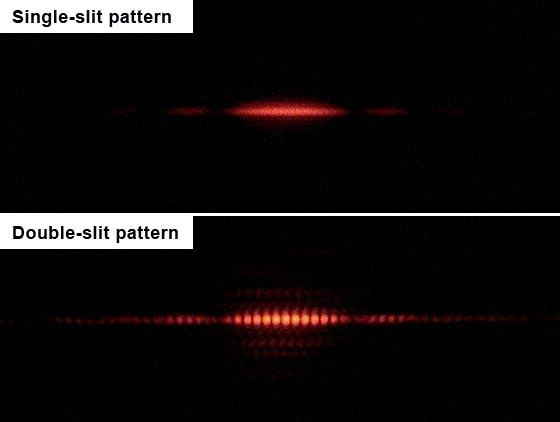
\includegraphics[width=4in]{image1.jpg}
\caption{Single and double-slit interference patterns \cite{wik}.}

\includegraphics[width=4.5in]{white.png}
\label{image}
\end{figure}

\maketitle 

%____________Introduction____________________________________________
\section{Introduction}
The double-slit experiment, also know known as the Young$^\prime$s experiment, explores the wave-like nature of light. It is important in this experiment for the two sources of light are coherent and have the same phase. Back in 1801, Thomas Young had difficulty with using common light sources, such as candles and lanterns, to be served as coherent sources of light. Thus instead, Young performed the experiment by filtering sunlight through a pinhole in a window shutter split by a piece of card and projecting it horizontally across the room. Light waves from either side of the card coming through the pinhole can be thus considered coherent sources and the interference pattern was then projected onto a screen from which the wavelength of the light source could be determined using Young$^\prime$s Equation: $$\lambda=\frac{y d}{m L}$$

Today, we can do the experiment by using the TWS apparatus that includes a monochromatic laser beam at one end (with a wavelength of 670 nm) passing through a double slit all encapsulated in a tightly sealed u-channel. Adjusting the micrometer attached to the detector-slit allows you to gather information regarding the interference pattern that is projected to a photodiode at the other end of the u-channel.

%____________Experiment____________________________________________
\section{Experiment}
In this experiment, the apparatus is set up as shown in Fig. \ref{dia}. After precise alignment of the laser, the double-slit, the slit-blocker, and the detector-slit, the photodiode is connected to a multimeter which is ultimately connected to the computer. LabView is used to collect data first for the double-slit experiment and for the single-slit experiment. \\

\begin{figure}[h!]
\centering
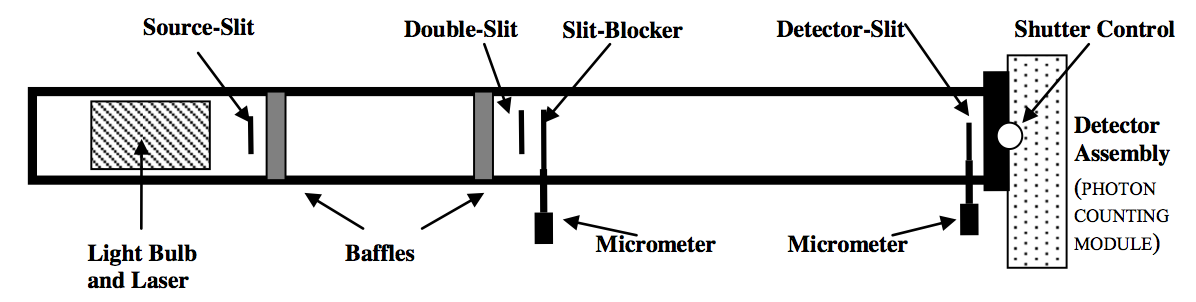
\includegraphics[width=7in]{dia}
\caption{Schematic of TWS apparatus - not to scale \cite{dia}.}
\label{dia}
\end{figure}
All parts are carefully aligned and key positions of the slit-blocker are recorded, so that light from one or two slits could be blocked and form both double-slit and single-slit interference patterns. The shutter at the end of the U-channel was kept closed, because only the photodiode on the surface of the shutter is used. After the preparation work, the double-slit experiment is first performed. A double-slit of slit width approximately 0.1 mm and slit separation 0.406 mm is used. \\

The slit-blocker is set at the position where light from both slits are allowed to pass, and the detector-slit is set at the position of the central maximum. The photodiode outputs a voltage that is proportional to the intensity of the laser beam. \\ 

By changing the position of the detector-slit, intensity of the laser light is recorded by LabView as a function of location. Then the experiment is repeated for single-slit when the slit-blocker blocks light from one of the two slits. \\
%____________Results____________________________________________
\section{Results}

\begin{figure}[h]
\centering
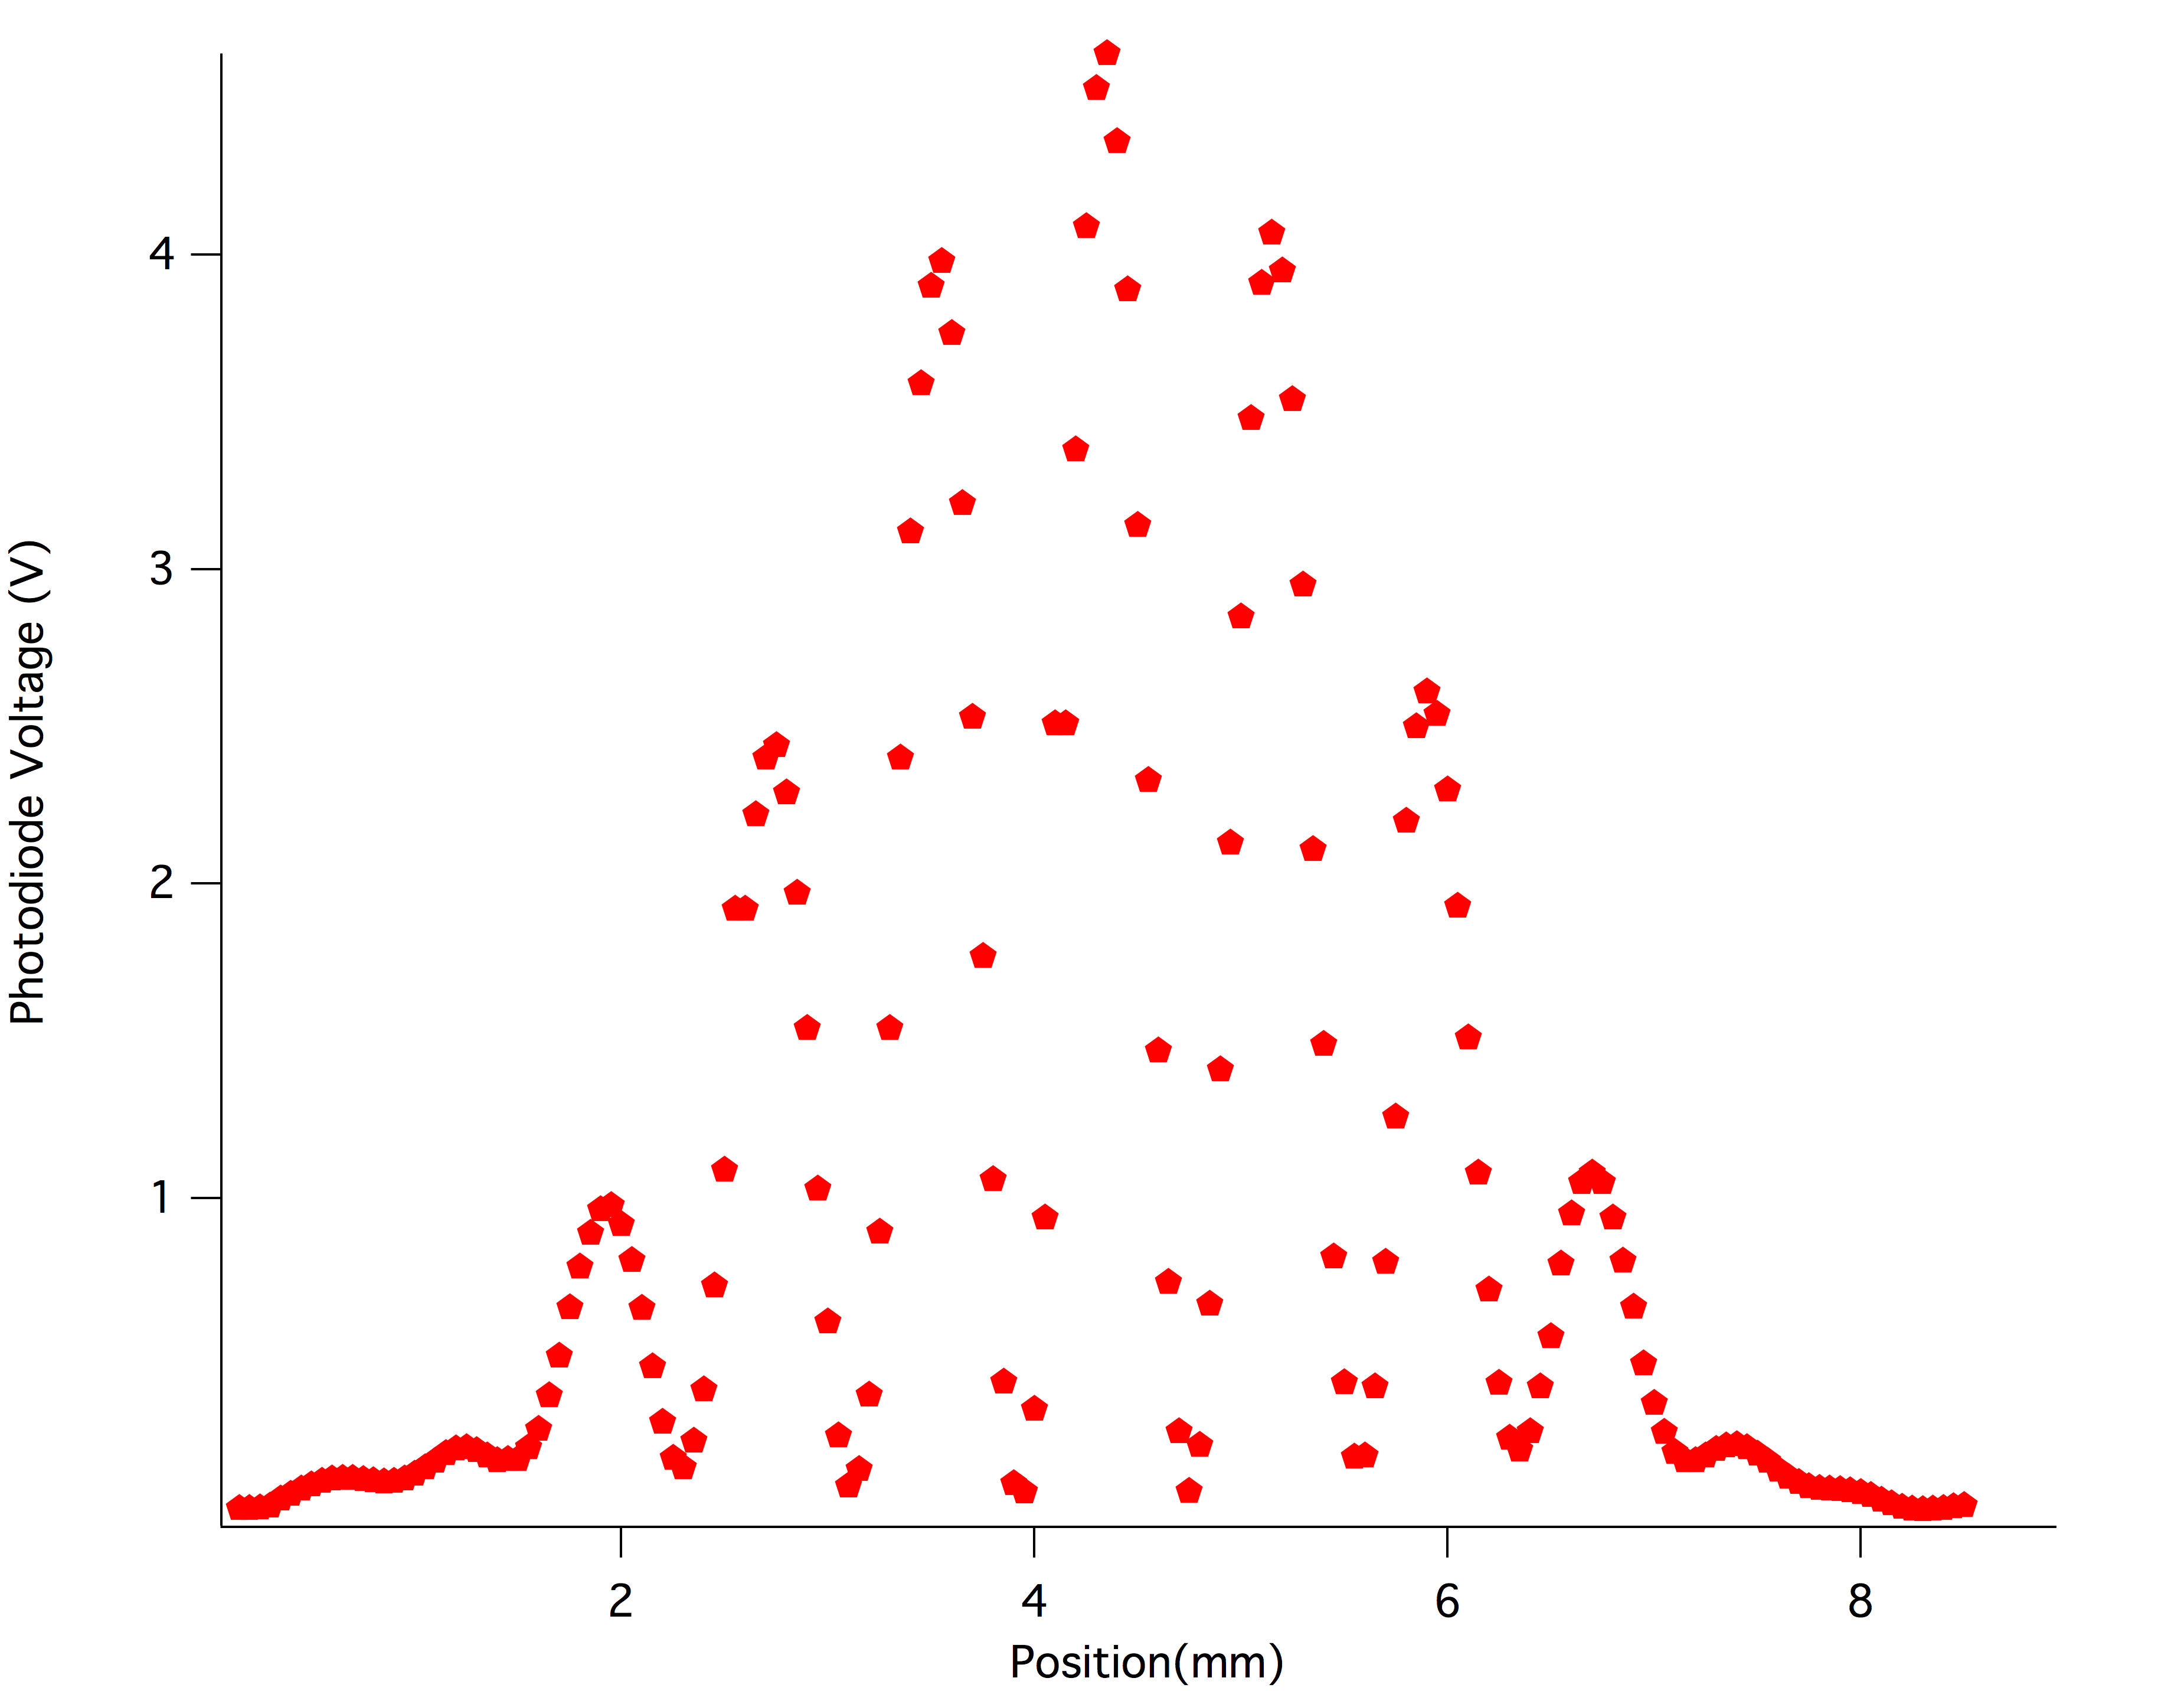
\includegraphics[width=3.2in]{doubleres.png}
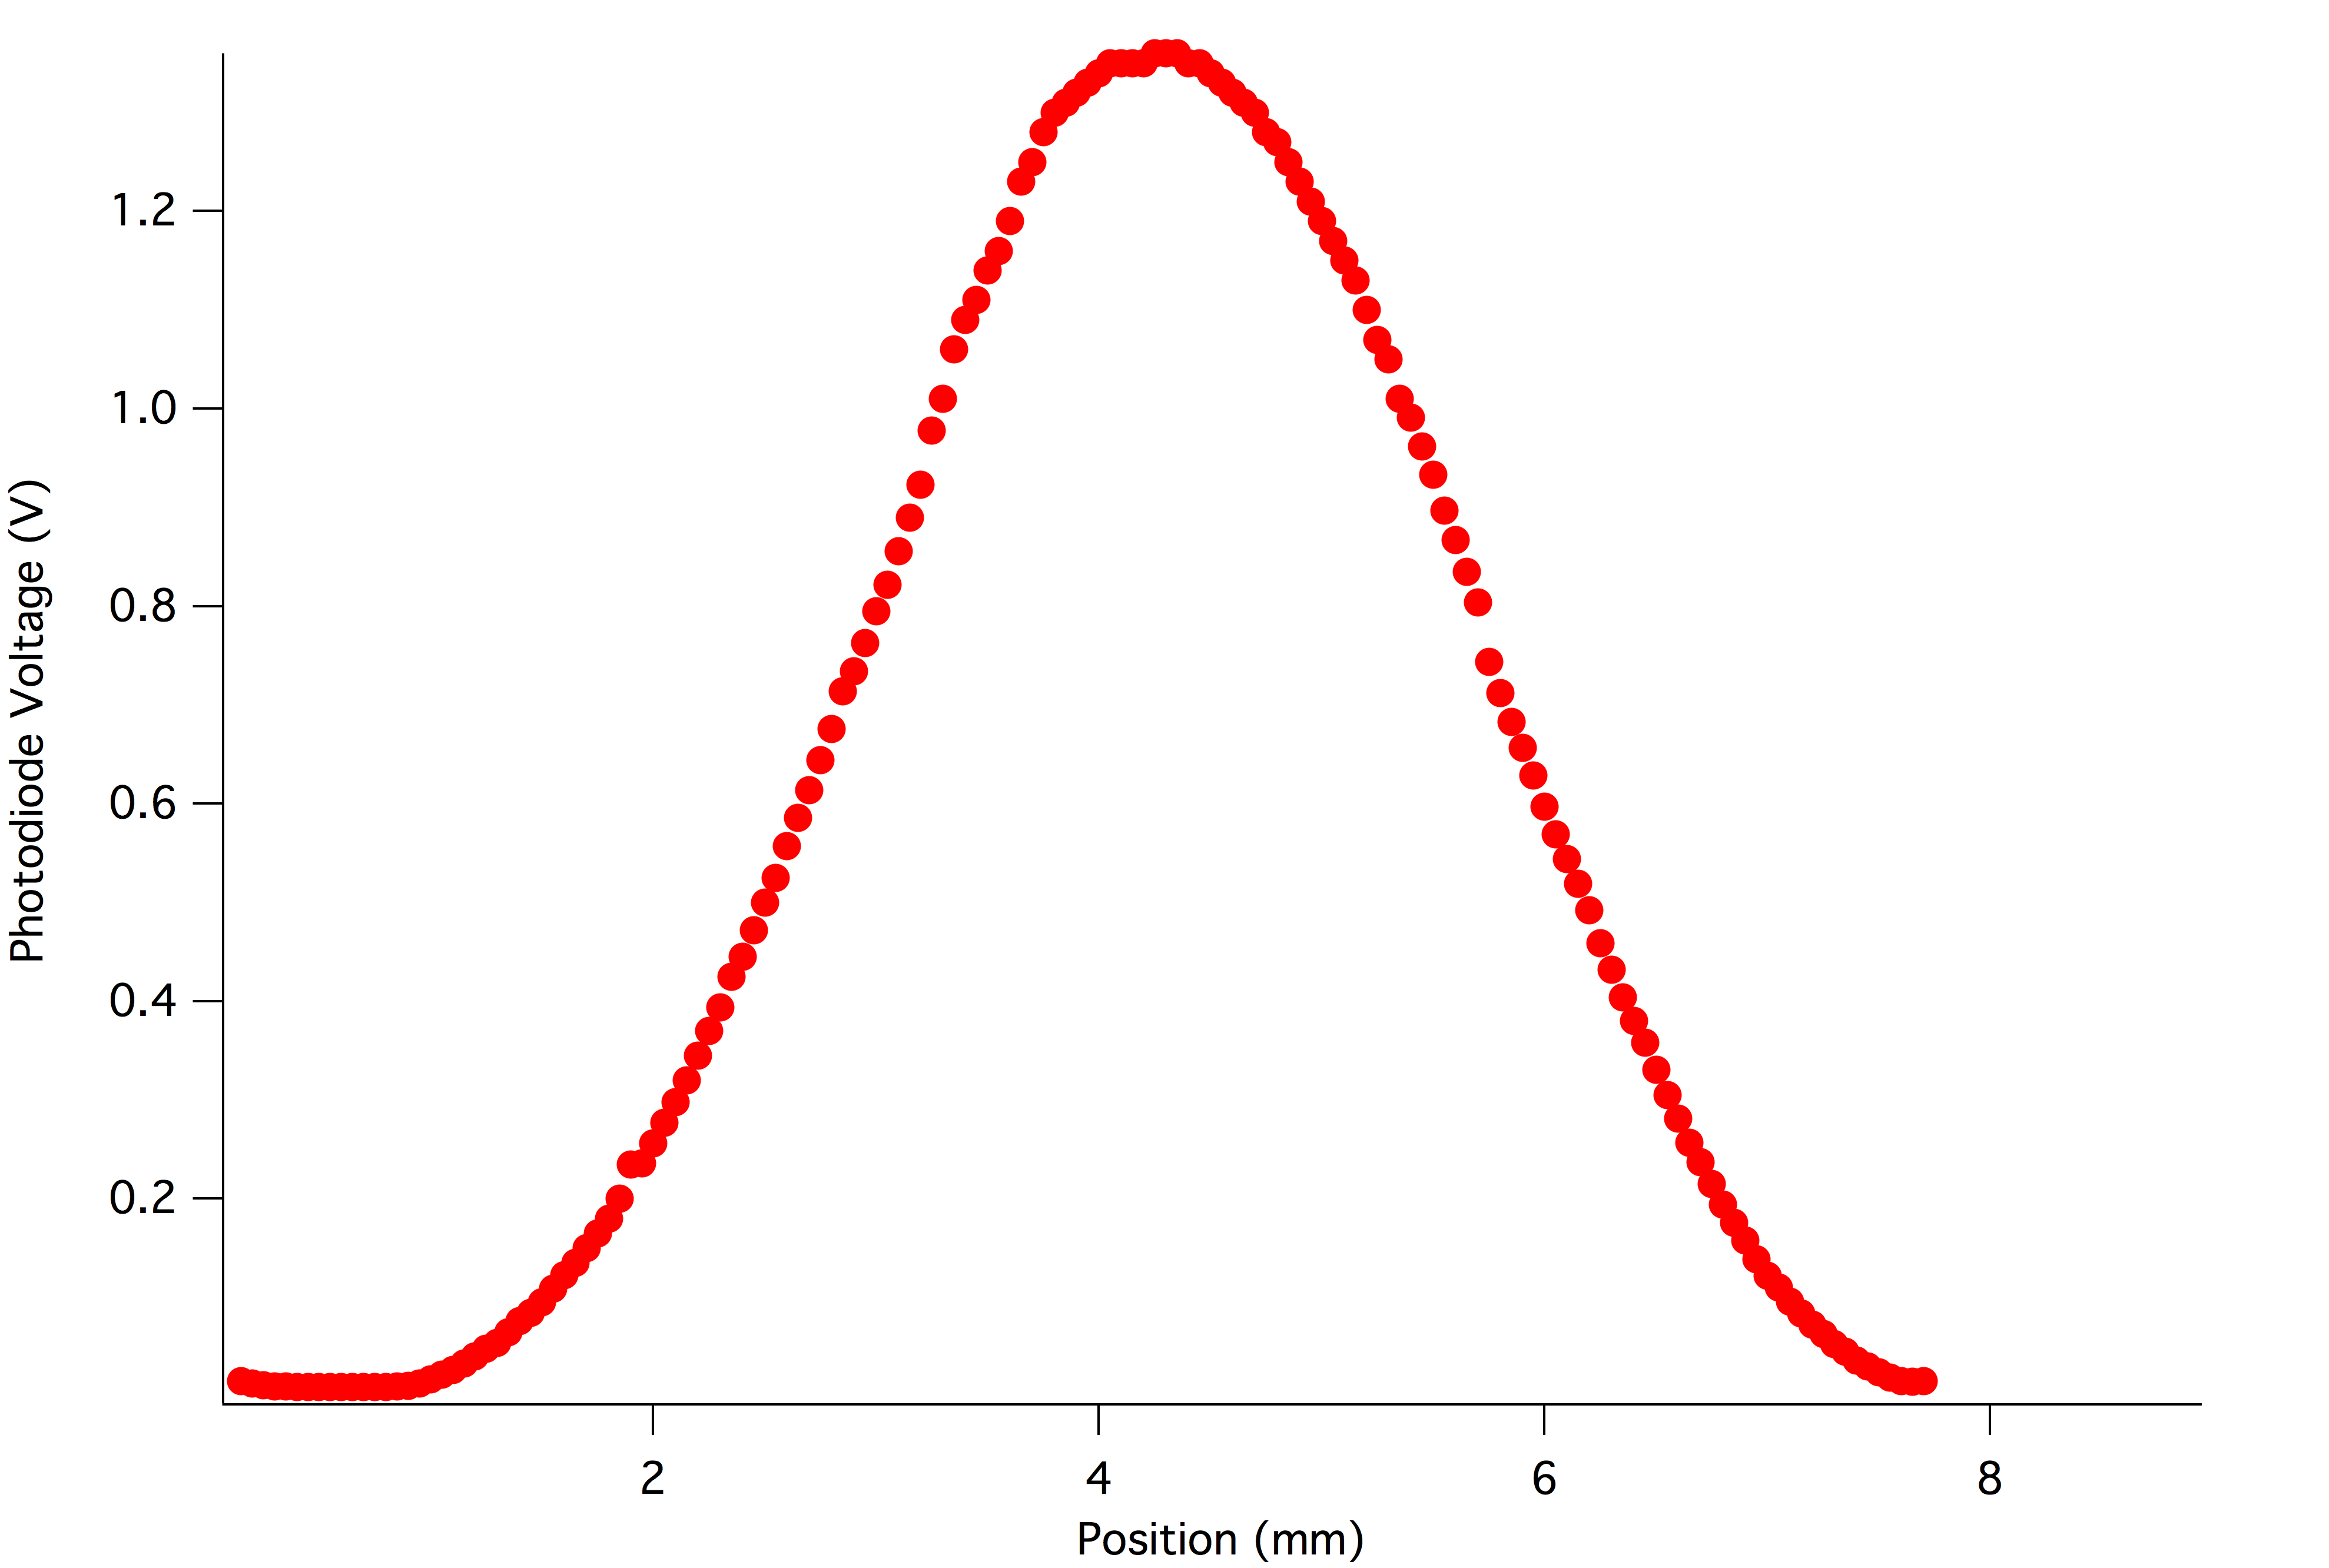
\includegraphics[width=3.2in]{singleres.png}
\caption{Recorded data for double (left) and single-slit (right) interference experiments.}
\label{ds}
\end{figure}

\newpage

The recorded raw data for the double and single-slit experiments are shown in Fig.\ref{ds}. First looking at the double slit experiment, to create the curve of best fit, the Fraunhofer equation is applied to the double-slit intensity: 

\begin{equation}
I=I_0 sinc^2( \frac{\pi a}{\lambda} sin \theta)  cos^2(\frac{\pi d}{\lambda} sin \theta)
\label{eq1}
\end{equation}

Using plotting tools in Igor while applying Eq. \ref{eq1}, we can obtain the plot shown below in Fig. \ref{double}. Calculation of the error bars will be included in the discussion section.

\begin{figure}[h]
\centering
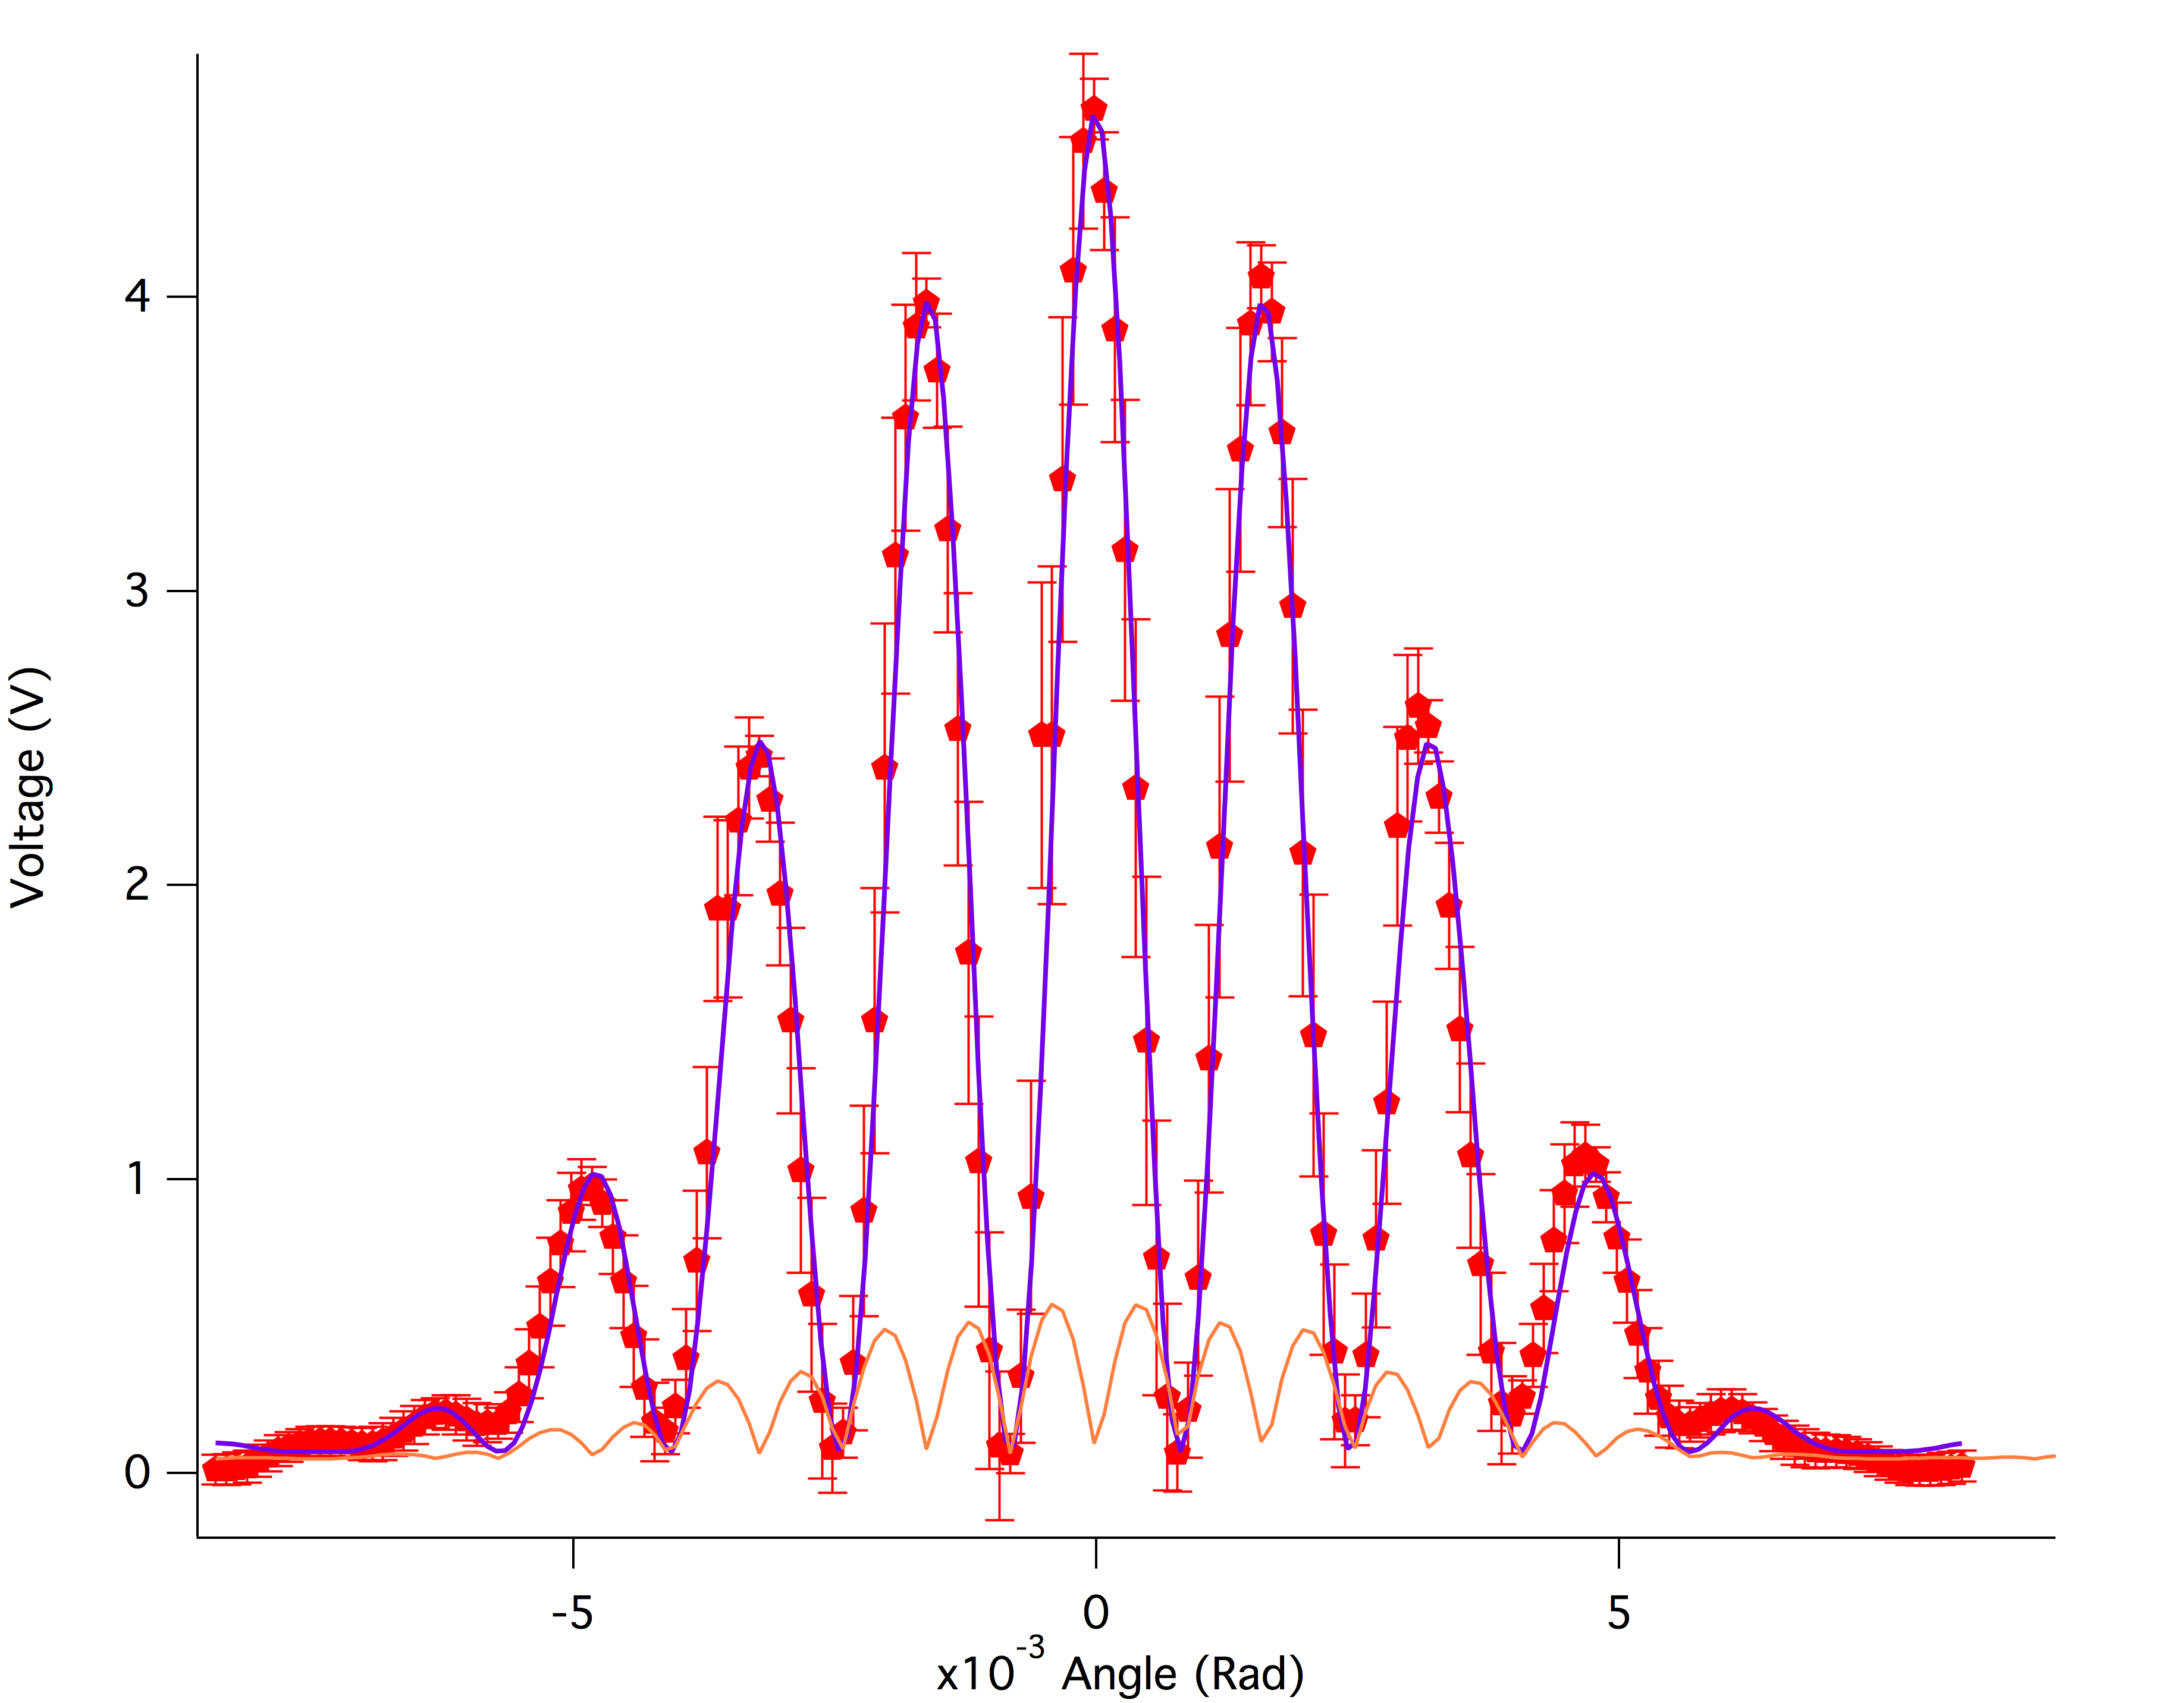
\includegraphics[width=7in]{double.png}
\caption{Plot of double-slit interference.}
\label{double}
\end{figure}

\begin{table}[h]
\centering
\caption{Double-slit data}
\begin{ruledtabular}
\begin{tabular}{ l c c c}
Name & Symbol & Value & Uncertainties($\pm$)\\
\hline
Slit width & a & 88.26 $\mu m$ & 0.384 $\mu m$\\
Slit separation & d & 426.89 $\mu m$ & 0.066 $\mu m$\\
Wavelength & $\lambda$ & 0.67 nm & 0\\
Max voltage & $V_0$ & 4.5532 V & 0.066 V\\
Voltage offset & $V_{offset}$ & 0.073317 V & 0.0075 V\\
Theta offset &$ \theta_{offset}$ & 1E-05 rad & 7.57e-06 rad \\
\hline
Chi Squared & $X^2$ & 0.827068&
\end{tabular}
\end{ruledtabular}
\label{data}
\end{table}

\newpage

The Fraunhofer conditions can be applied once again to create  the curve of best fit for the single-slit experiment: 
\begin{equation}
I=I_0 sinc^2 (\frac{\pi a}{\lambda} sin\theta)
\label{eq2}
\end{equation}

\begin{figure}[h]
\centering
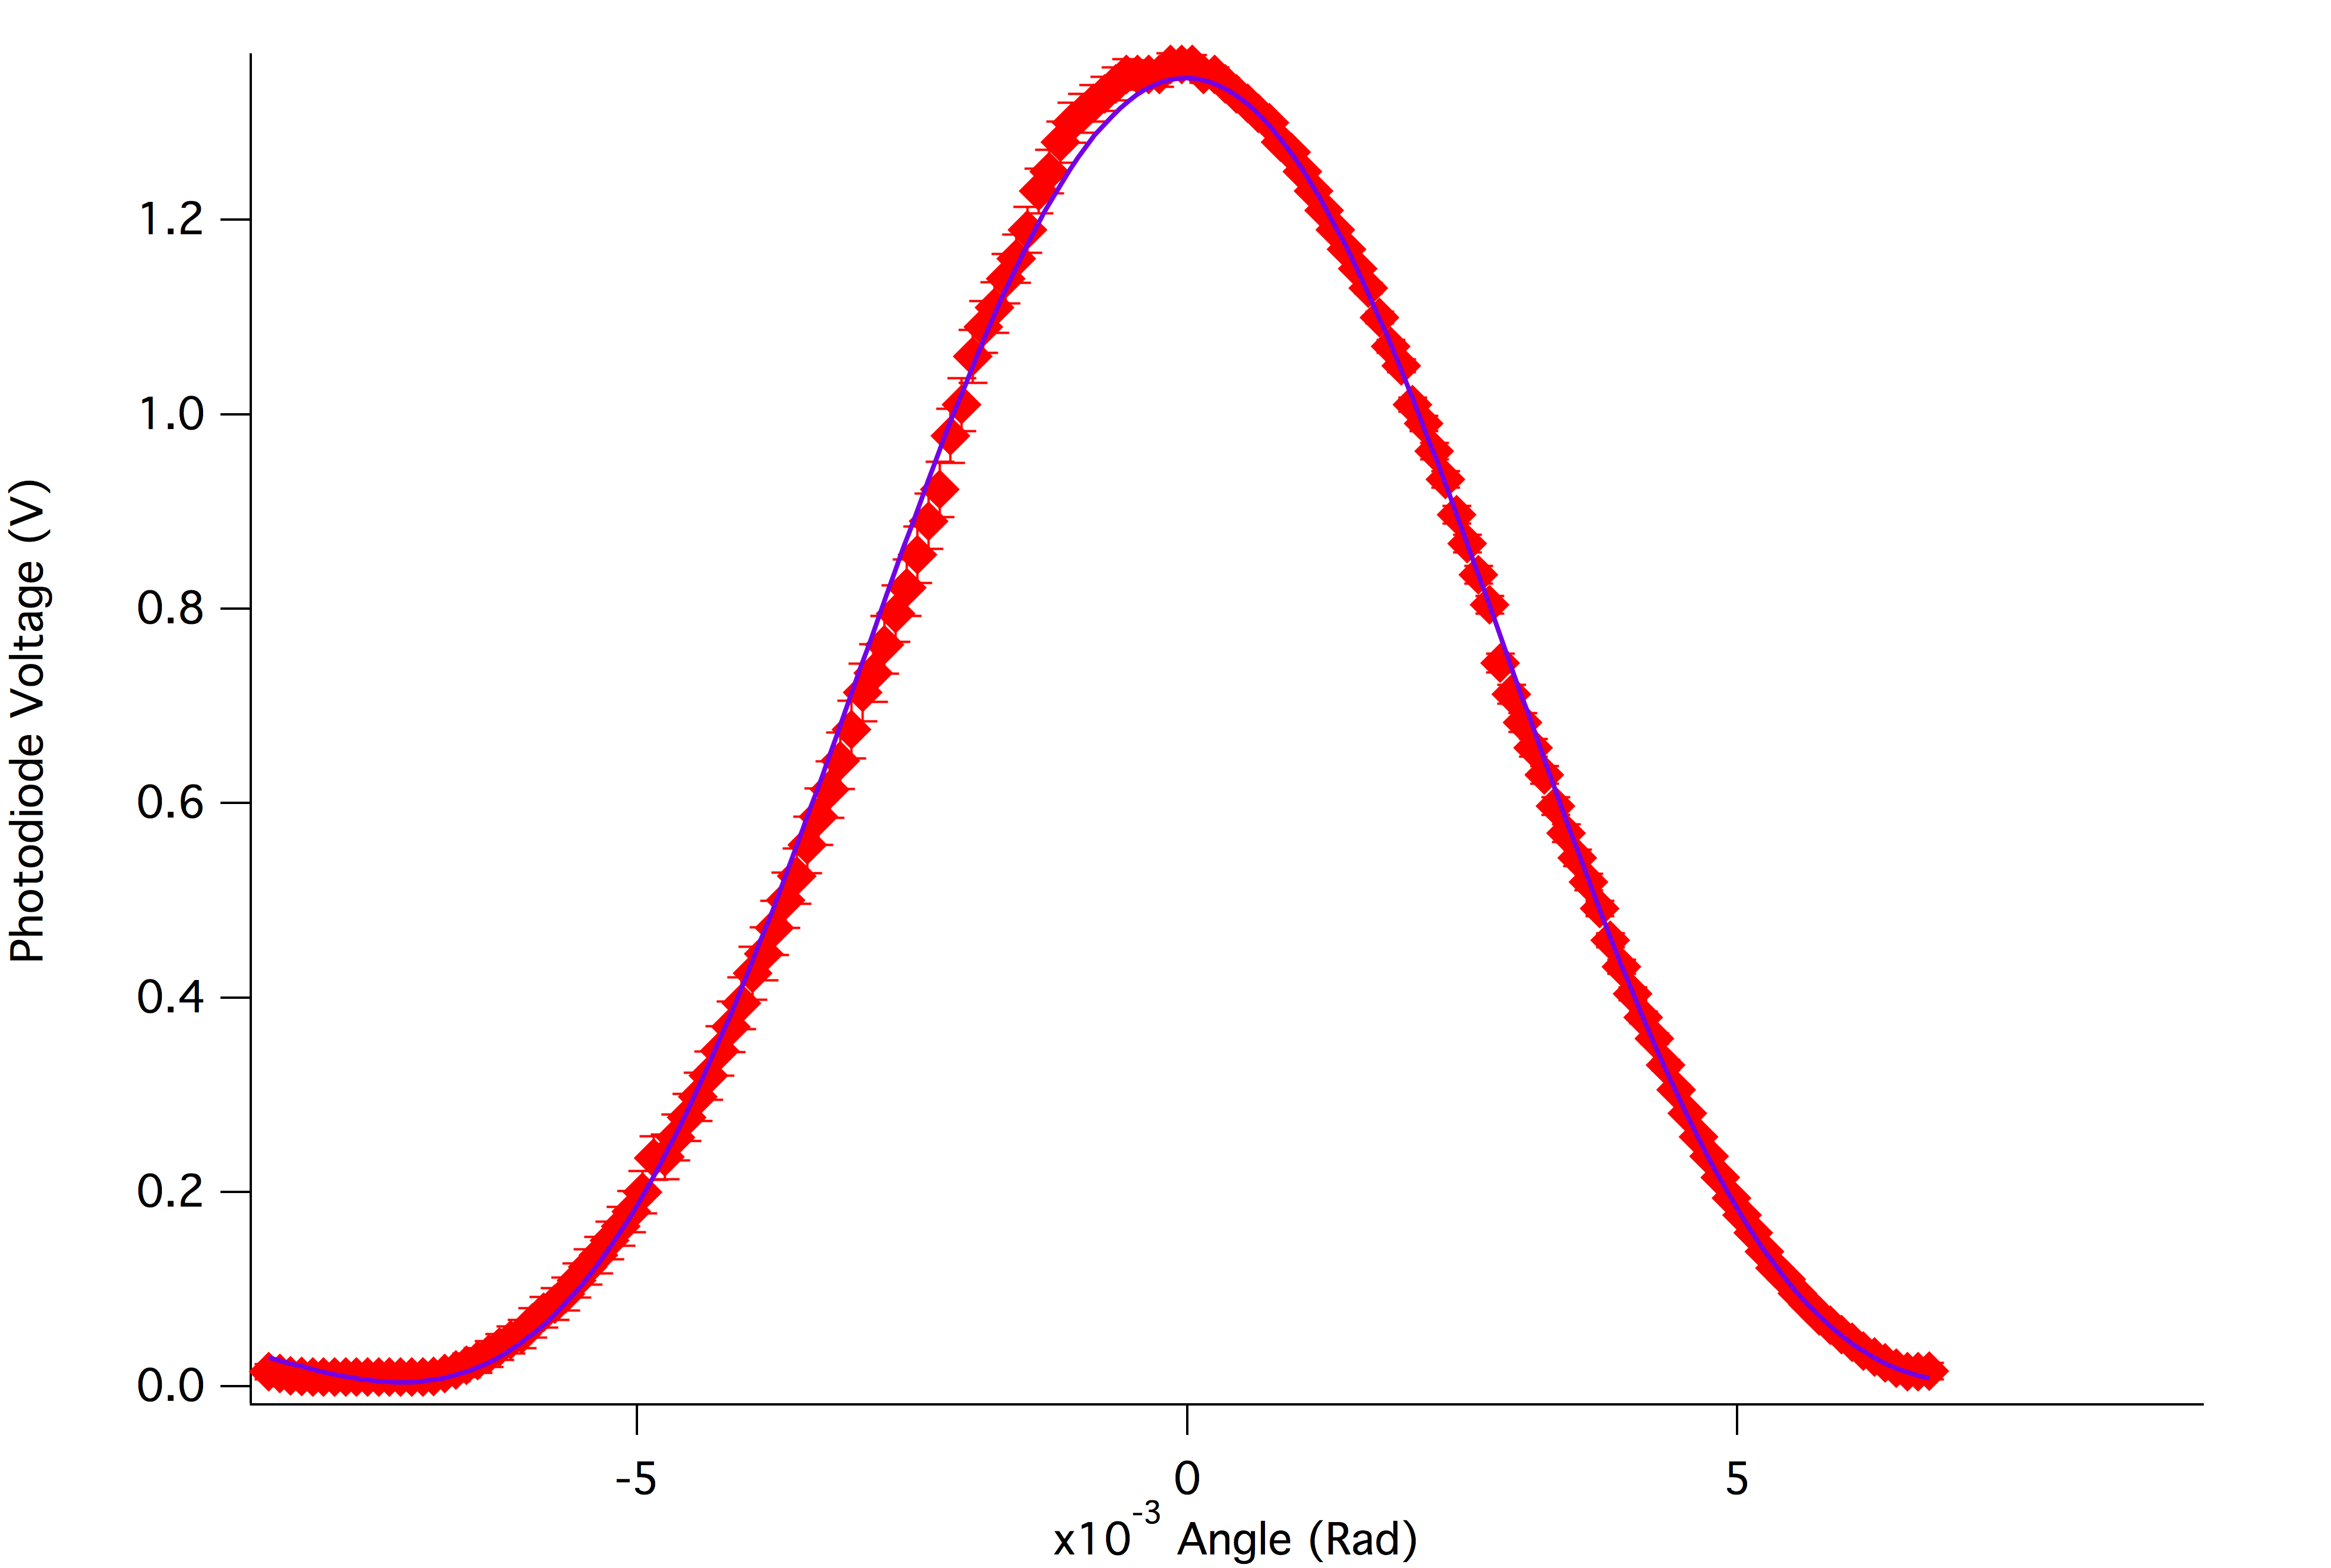
\includegraphics[width=6.6in]{single.png}
\caption{Plot of single-slit interference.}
\label{single}
\end{figure}

Using plotting tools in Igor while applying Eq.\ref{eq2}, we can obtain the plot shown in Fig.\ref{single}. Calculation of the error bars will be once again included in the discussion section for the single slit experiment.

\begin{table}[h]
\centering
\caption{Single-slit data}
\begin{ruledtabular}
\begin{tabular}{ l c c c}
Name & Symbol & Value & Uncertainties($\pm$)\\
\hline
Slit width & a & 88.008 $\mu m$ & 0.0954 $\mu m$\\
Wavelength & $\lambda$ & 0.67 nm & 0\\
Max voltage & $V_0$ & 1.3583 V & 0.00113 V\\
Voltage offset & $V_{offset}$ &  V &  V\\
Theta offset &$ \theta_{offset}$ & -05 rad & -06 rad \\

\hline
Chi Squared & $\chi^2$ & 2.44549&
\end{tabular}
\end{ruledtabular}
\label{data}
\end{table}

%____________Discussion____________________________________________
\section{Discussion}

\subsection{Double-Slit Experiment}

The Fraunhofer/Fresnel theory (Eq.\ref{eq1}) of interference gives the intensity of light as a function of angle. The photodiode we use to conduct the experiment outputs a voltage proportional to the intensity of light detected ($I = kV$), thus the intensity measurements can be replaced by the voltage readings and the analysis holds for both:

\begin{equation}
V=V_0 sinc^2( \frac{\pi a}{\lambda} sin (\theta+\theta_{offset}))  cos^2(\frac{\pi d}{\lambda} sin (\theta+\theta_{offset}) + V_{offset}
\label{fitdouble}
\end{equation}

Several parameters are added to the original Fraunhofer model. $V_{offset}$ is describing the affect of the background light. Although the photodiode is kept in a closed black box, there is a slight amount of background light, which will produce an offset and shift the whole curve up. $\theta_{offset}$ describes the systematic error in angle, which is a result of the systematic error in position.\\

Some other parameters need fitting are slit width and slit separation. Due to manufacturing imperfection, the slit width and slit separation have slightly different values than given by the experiment manual. The wavelength of the laser might also be slightly off, but because equation m contains ratio terms $\frac{\pi a}{\lambda}$ and $\frac{\pi d}{\lambda}$, the numerator and denominator cannot change at the same time. Compared to a and d, $\lambda$ is less likely to have a greatly different value, so it is held at 0.67 $\mu m$. $V_{0}$ stands for the voltage measured at the central maximum.\\

Uncertainty in the variable (angle $\theta$) is determined by applying error propagation. Each step of the detector-slit change is designed to be 0.05 mm on the micrometer, from $x_i = 0.15 mm$ to $x_f = 8.35 mm$. Angle $\theta$ corresponds to the position in radian is given by
\begin{equation}
\theta = \frac{arctan(x-x_0)}{D}
\label{theta}
\end{equation}
$D$ is the distance from the double-slit to the photodiode, is 50 cm given by the experiment manual.
$x_0$ is found to be 4.3627 mm given by the Gaussian curve fit to the data set.

\begin{figure}[h]
\centering
\includegraphics[width=7in]{doublegaus.pdf}
\caption{Gaussian curve fit of double-slit interference.}
\label{gasfit}
\end{figure}

However, due to human error, each step is not perfectly 0.05 mm, but $0.05\pm0.03 mm$.
Then the error in angle is given by taking derivative of equation n and multiply theta prime by delta x, which is 0.03. 
[theta prime equation]
Delta theta is a function of position x. The same method of taking derivative could be applied to find the error in voltage, but it is rather messy. So a different approach is adopted to find delta V, which is to change theta in equation m by delta m and calculate the resulting change in V, which is then divided by 2.
[delta V = abs (I(theta + delta theta) - I(theta - delta theta))/2]
It can be seen that delta theta has a smaller impact on delta V when V prime is small, and a bigger impact when V prime is big.\\

The multimeter itself also contributes to the error in angle. We estimate the error in meter readings to be 0.05v.
So the overall delta V is
[delta V = abs (I(theta + delta theta) - I(theta - delta theta))/2 + 0.05v]
Delta V is plotted as a function of angle in the figure.\\

After the curve fitting, a chi squared evaluation is done, and yields a chi square of something, which is close to 1, meaning that the estimation for error is reasonable. \\





\subsection{Single-Slit Experiment}

Section 2 Single-Slit Experiment
The intensity of light as a function of theta in single-slit experiment is given by the Fraunhofer/Fresnel theory
[I(theta) = equation]
Parameters need fitting are slit width, slit separation, maximal voltage, offset in voltage due to background light, and offset in theta due to systematic error of position.

Uncertainty is determined using the same method.
[theta = arctan((x-x0)/distance)] {equation p}
The position of the central maximum of the single-slit pattern is slightly shifted than that of the double-slit pattern, so a gaussian fit is added to the data to find out the offset in x.
[figure]
The distance is still 50 cm.
Step size, delta x





%____________Conclusion____________________________________________
\section{Conclusion}



\begin{acknowledgments}

We gratefully acknowledge Nathaneal Fortune and Dana Parsons, who helped with the experimentation and editing of this experiment.  This work was supported by the Smith College Physics Department.

\end{acknowledgments}


\begin{thebibliography}{99}

\bibitem{wik} Double Slit Experiment, \url{<http://upload.wikimedia.org/wikipedia/commons/c/c2/Single_slit_and_double_slit2.jpg
/>}.

\bibitem{dia} TeachSpin Instructions Manual,\textit{Two-Slit interference, One Photon at a Time (TWS1-B), Pulse Counter/Interval Timer (PCIT1)}, 6/2013.

\end{thebibliography}

%\newpage   % Start a new page for tables

\end{document}
